%=====================================
% Author: Christian Fischer Pedersen
% About: Slide template
%=====================================
%==============================
%   Author: Christian Fischer Pedersen
%   About: Beamer style file
%==============================

%========General
\documentclass[compress,mathserif,presentation,notheorems]{beamer}
%\usepackage[export]{adjustbox}
\usepackage{etex}
\usepackage[utf8]{inputenc}%Danske bogstaver
\usetheme{default}
\usecolortheme{default}

%========Fonts
\setbeamercolor{structure}{fg=aaudblue}
\setbeamerfont{structure}{family=\sf\bfseries}
\setbeamercolor{normal text}{fg=black}
\setbeamerfont{normal text}{family=\sf\mdseries}
\renewcommand{\footnoterule}{}
\renewcommand{\footnotesize}{\tiny}

%========Sections
\AtBeginSection[]{\begin{frame}\frametitle{Outline}\tableofcontents[currentsection]\end{frame}}

%========Parts
\makeatletter
\AtBeginPart{%
  \addtocontents{toc}{\protect\beamer@partintoc{\the\c@part}{\beamer@partnameshort}{\the\c@page}}%
}
%% number, shortname, page.
\providecommand\beamer@partintoc[3]{%
  \ifnum\c@tocdepth=-1\relax
    % requesting onlyparts.
    \sf{\bf{\textcolor{aaudblue}{\makebox[6em]{PART #1:}#2}}}
    \par
  \fi
}
\define@key{beamertoc}{onlyparts}[]{%
  \c@tocdepth=-1\relax
}
\makeatother

%========Itemize and enumerate
\setbeamertemplate{itemize items}[triangle]%triangle,circle,ball,square
\setbeamertemplate{note page}[plain]

%========Colors
\usepackage{pstricks,pst-node}
\newrgbcolor{aaudblue}{0.2 0.4 0.6}   %dark blue
\newrgbcolor{aaulblue}{0.4 0.6 0.8}   %light blue
\newrgbcolor{lgray}   {0.9 0.9 0.9} %light gray
\definecolor{lgray}{rgb}{0.9,0.9,0.9} %light gray
\definecolor{mgray}{rgb}{0.5,0.5,0.5} %medium gray
\definecolor{dgray}{rgb}{0.2,0.2,0.2} %dark gray

%========Footer
\beamertemplatenavigationsymbolsempty
\usepackage{tabularx}
\setbeamertemplate{footline}{
%\colorbox{white}
{\color{aaudblue}
\begin{tabularx}{0.98\textwidth}{l X}
~\insertshortauthor, \insertshortinstitute & \hfill \insertframenumber$|$\inserttotalframenumber\\
\end{tabularx}
}\vskip6pt
}

%========Header
\setbeamercolor*{palette tertiary}{fg=aaudblue,bg=white}
\setbeamertemplate{headline}{%
\begin{beamercolorbox}{section in head/foot}
\vskip6pt \insertsectionnavigationhorizontal{\paperwidth}{}{} \vskip2pt
%\vskip6pt \insertnavigation{\paperwidth} \vskip2pt
\end{beamercolorbox}%
}

%========Title page
\newcommand{\slidetitlepage}[2]{
\title{#1}
\subtitle{#2}
\author[Christian Fischer Pedersen]%
{Christian Fischer Pedersen\\[-1.4mm]%
%{\scriptsize Associate Professor, PhD}\\[-1.4mm]%
{\scriptsize cfp@eng.au.dk}}
\institute[Electrical and Computer Engineering, Aarhus University]%
{Section of Electrical and Computer Engineering\\
Department of Engineering\\
Aarhus University}
\date{{\scriptsize Revised on \today}}
}


%========Math fonts 
\usepackage{amsmath}
\usepackage{bbm}
\usepackage{pifont}
\usepackage{wasysym}
\usepackage{amssymb}
\usepackage{amsbsy}


%========Blocks
\setbeamertemplate{blocks}[rounded][shadow=true]
\setbeamercolor{block title} {bg=aaulblue,fg=white}
\setbeamercolor{block body}{bg=white,fg=black}%fg=lgray}

%========Figures and graphics
\usepackage[dvips]{epsfig}
\usepackage[dvips]{graphicx}
\usepackage{subfigure}
\usepackage{caption}%Skal komme efter 'subfigure' for ogsaa at virke paa denne
\usepackage{fancybox}\cornersize{1}
\usepackage{tikz}


%========Video and sound
%\usepackage{multimedia}


%========Tables
%\usepackage{booktabs}
\usepackage{rotating}
\usepackage{multirow}


%========Referencing and citations
\usepackage[sort&compress, numbers]{natbib}
\newcommand{\citefont}[1]%
{\fontsize{5pt}{5pt}\selectfont#1\normalsize}

\newcommand{\scite}[1]%Formerly known as "slidecite"
{\fontsize{5pt}{5pt}\selectfont(\citeauthor{#1}, \citeyear{#1} [\citenum{#1}])\normalsize}

\newcommand{\sciten}[1]%Formerly known as "slidecitenormal"
{(\citeauthor{#1}, \citeyear{#1} [\citenum{#1}])}

\newcommand{\scitennp}[1]%Formerly known as "slidecitenormalnp" - np means no parantheses 
{\citeauthor{#1}, \citeyear{#1} [\citenum{#1}]}

\newcommand{\scitesub}[1]%Formerly known as "slidecitesubmitted"
{\fontsize{5pt}{5pt}\selectfont(\citet{#1})\normalsize}

\renewcommand{\bibsection}{\subsubsection*{\bibname}} %Avoid 'References' in header

\newcommand{\shref}[2]%
{\href{#1}{\textcolor{aaudblue}{\textbf{#2}}}}

%\bibpunct[:]{(}{)}{;}{a}{}{,}

%========Misc. defines
\newcommand{\nolinefrac}[2]{\genfrac{}{}{0pt}{}{#1}{#2}}
\def\simiid{\overset{\scriptsize{i.i.d.}}{\sim}}
\def\CSMfac{$\textrm{CSM}_{\textrm{fac}}~$}
\def\CSMfft{$\textrm{CSM}_{\textrm{fft}}~$}
\def\Matlab{Matlab$^\copyright~$}
\def\rhoot{\mbox{\large{$\varrho$}}}

%========Vectors and matrices
\def\lambdav{\boldsymbol{\lambda}}
\def\lambdam{\mathbf{\Lambda}}
%\newcommand{\tlv}[1]{\tilde{\lv}^{{\raisebox{-2pt}{\footnotesize $(#1)$}}}} 
\def\deltav{\boldsymbol{\delta}}
\def\deltam{\mathbf{\Delta}}

%========Listings
\usepackage{listings}
% \lstset{
% nputencoding=T1,
% language=Matlab,
% xleftmargin=8pt,
% tabsize=2,
% basicstyle=\small, print whole listing small
% keywordstyle=\color{black}\bfseries, 
% identifierstyle=, nothing happens
% commentstyle=\color{black}\itshape,
% stringstyle=\color{black}\ttfamily,
% showstringspaces=false,
% numbers=left,
% stepnumber=0,
% numbersep=4pt,
% morekeywords={display}
% }

%Theorem environments
%----------------------------------------------------------
\usepackage{amsthm}
\theoremstyle{remark}
%\theoremstyle{definition}
\newtheorem{theorem}{Theorem}
\newtheorem{acknowledgement}{Acknowledgement}
\newtheorem{algorithm}{Algorithm}
\newtheorem{axiom}{Axiom}
\newtheorem{case}{Case}
\newtheorem{claim}{Claim}
\newtheorem{conclusion}{Conclusion}
\newtheorem{condition}{Condition}
\newtheorem{conjecture}{Conjecture}
\newtheorem{corollary}{Corollary}
\newtheorem{criterion}{Criterion}
\newtheorem{definition}{Definition}
\newtheorem{example}{Example}
\newtheorem{exercise}{Exercise}
\newtheorem{lemma}{Lemma}
\newtheorem{notation}{Notation}
\newtheorem{problem}{Problem}
\newtheorem{proposition}{Proposition}
\newtheorem{remark}{Remark}
\newtheorem{solution}{Solution}
\newtheorem{summary}{Summary}
\newtheorem{property}{Property}
\newtheorem{equivalence}{Equivalence}
\newtheorem{expression}{Expression}
%\setbeameroption{show notes} un-comment to see the notes

%===============Title slide
\slidetitlepage{Cloud Computing, Part 2}{Distributed and Pervasive Systems, MSc}

\begin{document}
\begin{frame}[plain]
\titlepage
\end{frame}

%===============Outline slide: Parts
\begin{frame}
\frametitle{Outline}
\tableofcontents
\end{frame}

%===============Slides
\section[Recap]{Recap}
\frame{
	\frametitle{From last time}
	\framesubtitle{}
	What did we learn?
	\begin{itemize}
		\item Cloud computing is delivery of online computing services
		\item Microservices are SoA-styled small, independent services that do one thing
		\item Containers are lightweight isolated software environments
		\item Docker is a container tool that can run and create containers
		\item Kubernetes is an open-source container orchestration engine
	\end{itemize}
}

\section[Pods]{Pods}
\frame{
	\frametitle{Pods in Kubernetes}
	\framesubtitle{}
	What is a pod?
	\begin{itemize}
		\item A pod is a group of one or more tightly\\
		related containers that run together and share namespace
		\item Each pod is like a separate logical machine.
		\item All containers in a pod will appear to be\\
		running on the same logical machine.
		\item Can only run on one node
	\end{itemize}
	\begin{figure}[htbp!]
		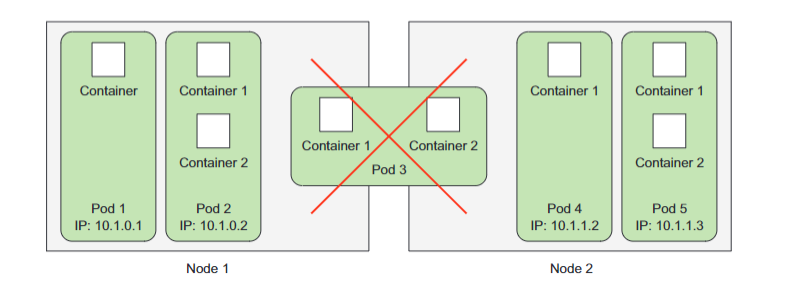
\includegraphics[width=0.8\textwidth]{figures/3_1.png}
		\caption{Fig. by courtesy of Marko Luksa\cite{Luksa2018}}
		\label{fig:}
	\end{figure}
}

\frame{
	\frametitle{Why pods?}
	\framesubtitle{}
	\begin{itemize}
		\item Containers run only a single process.
		\item Pods allow us to bind containers together as a single unit.
		\item Pods run closely related processes together in the same environment.
		\item Processes think they are running together. Closed world.
	\end{itemize}	
}

\frame{
	\frametitle{Network with pods}
	\framesubtitle{}
	\begin{itemize}
		\item All pods reside in a single flat, shared, network address space.
		\item Containers share the same IP
		\item Avoid port conflicts
	\end{itemize}
	\begin{figure}[htbp!]
		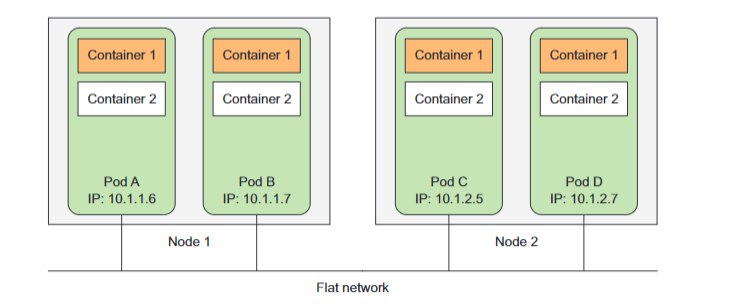
\includegraphics[width=1\textwidth]{figures/3_2.png}
		\caption{Fig. by courtesy of Marko Luksa\cite{Luksa2018}}
		\label{fig:}
	\end{figure}
}

\frame{
	\frametitle{The inside of a pod}
	\framesubtitle{}
	\begin{figure}[htbp!]
		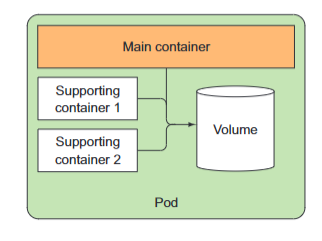
\includegraphics[width=0.7\textwidth]{figures/3_3.png}
		\caption{Fig. by courtesy of Marko Luksa\cite{Luksa2018}}
		\label{fig:}
	\end{figure}
}

\frame{
	\frametitle{Using multiple containers}
	\framesubtitle{}
	When to use multiple containers?
	\begin{itemize}
		\item Do they need to be run together?
		\item Do they scale together?
		\item Are they single components or one whole?
	\end{itemize}
	\begin{figure}[htbp!]
		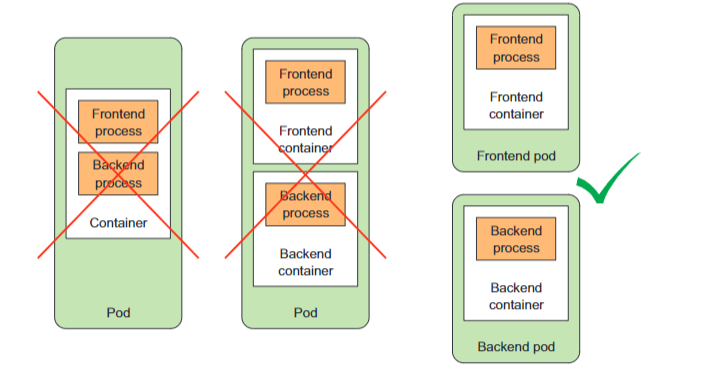
\includegraphics[width=0.8\textwidth]{figures/3_4.png}
		\caption{Fig. by courtesy of Marko Luksa\cite{Luksa2018}}
		\label{fig:}
	\end{figure}
}

\frame{
	\frametitle{Creating pods}
	\framesubtitle{}
	\begin{itemize}
		\item Created by posting a YAML or JSON to the Kubernetes API
		\item Instead of "kubectl run", you post a YAML file
		\item Enables more options and version control
	\end{itemize}
	\begin{figure}[htbp!]
		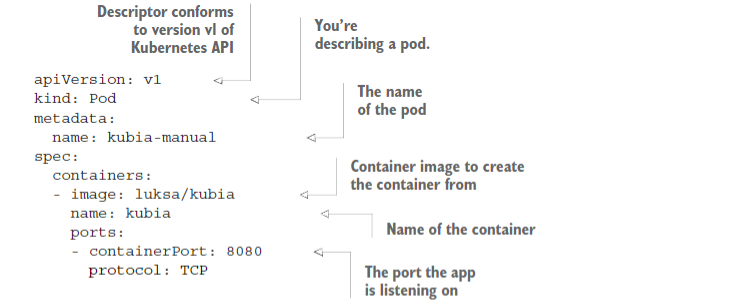
\includegraphics[width=1\textwidth]{listings/3_2.png}
		\caption{Listing by courtesy of Marko Luksa\cite{Luksa2018}}
		\label{fig:}
	\end{figure}
}

\begin{frame}[fragile]
	\frametitle{Creating pods commands}
	\framesubtitle{}
	Useful commands for creating pods and getting the manifest
	\begin{lstlisting}[numbers=none, basicstyle=\ttfamily]
$ kubectl create -f kubia-manual.yamlpod
$ kubectl get po kubia-manual -o yaml
$ kubectl get po kubia-manual -o json
$ kubectl get pods
$ kubectl logs kubia-manual
	\end{lstlisting}
\end{frame}

\begin{frame}[fragile]
	\frametitle{Connecting to pods}
	\framesubtitle{}
	Connect without a service
	\begin{lstlisting}[numbers=none, basicstyle=\ttfamily]
$ kubectl port-forward kubia-manual 8888:8080
... Forwarding from 127.0.0.1:8888 -> 8080
... Forwarding from [::1]:8888 -> 8080
$ curl localhost:8888
	\end{lstlisting}
	Note that minikube uses nodeIP:nodePort and not localhost:nodePort. Check with "minikube ip".
	\begin{figure}[htbp!]
		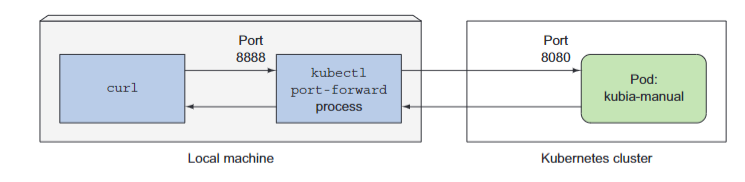
\includegraphics[width=1\textwidth]{figures/3_5.png}
		\caption{Fig. by courtesy of Marko Luksa\cite{Luksa2018}}
		\label{fig:}
	\end{figure}
\end{frame}

\frame{
	\frametitle{Organizing pods with labels}
	\framesubtitle{}
	\begin{itemize}
		\item Use labels to organize all Kubernetes resources.
		\item One or more labels
		\item Vertical and horizontal.
	\end{itemize}
	\begin{figure}[htbp!]
		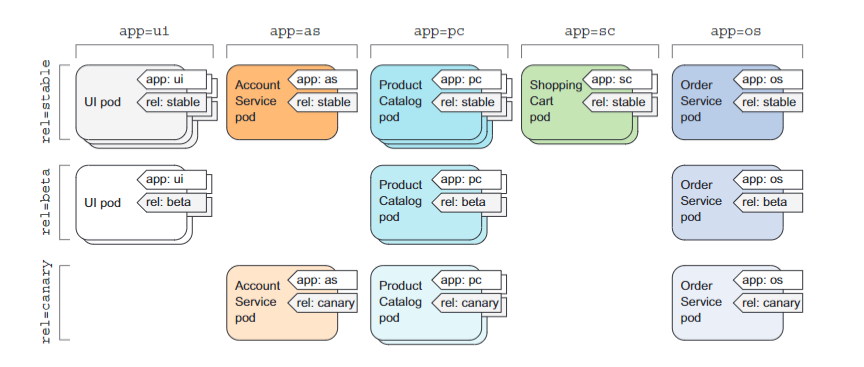
\includegraphics[width=1\textwidth]{figures/3_7.png}
		\caption{Fig. by courtesy of Marko Luksa\cite{Luksa2018}}
		\label{fig:}
	\end{figure}
}

\frame{
	\frametitle{Organizing pods with labels cont.}
	\framesubtitle{}
	\begin{figure}[htbp!]
		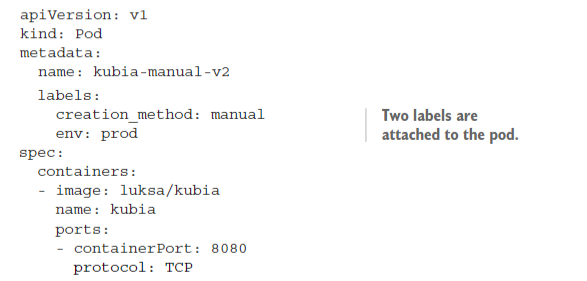
\includegraphics[width=1\textwidth]{listings/3_3.png}
		\caption{Listing by courtesy of Marko Luksa\cite{Luksa2018}}
		\label{fig:}
	\end{figure}
}

\begin{frame}[fragile]
	\frametitle{Organizing pods with labels cont.}
	\framesubtitle{}
	Create and show pods with labels
	\begin{lstlisting}[numbers=none, basicstyle=\ttfamily]
$ kubectl create -f kubia-manual-with-labels.yaml
$ kubectl get po --show-labels
$ kubectl get po -L creation_method,env
$ kubectl get po -l creation_method=manual
	\end{lstlisting}
	\begin{itemize}
		\item Dont worry about scheduling. Kubernetes handles that.
		\item Never say specifically what node a pod should run on.
	\end{itemize}
\end{frame}

\frame{
	\frametitle{Organizing pods with labels cont.}
	\framesubtitle{}
	\begin{figure}[htbp!]
		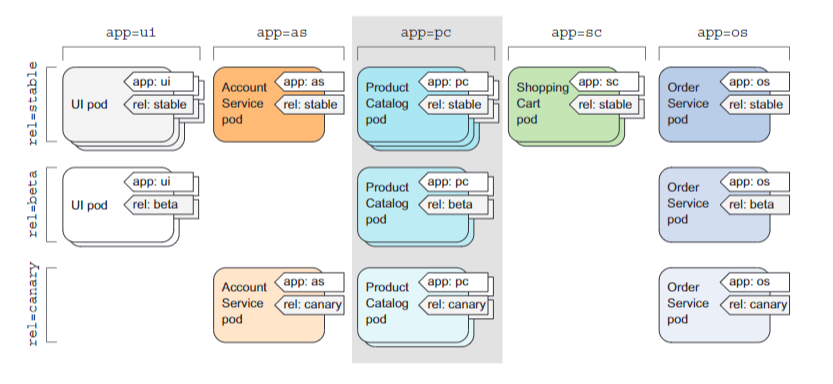
\includegraphics[width=1\textwidth]{figures/3_8.png}
		\caption{Fig. by courtesy of Marko Luksa\cite{Luksa2018}}
		\label{fig:}
	\end{figure}
}

\begin{frame}[fragile]
	\frametitle{Scheduling pods to specific nodes}
	\framesubtitle{}
	Not best practice, but it is possible
	\begin{lstlisting}[numbers=none, basicstyle=\ttfamily]
$ kubectl label node gke-kubia-85f6-node-0rrx
gpu=true
$ kubectl get nodes -l gpu=true
	\end{lstlisting}
	\begin{figure}[htbp!]
		
\includegraphics[width=1\textwidth]{listings/3_4.png}
		\caption{Listing by courtesy of Marko Luksa\cite{Luksa2018}}
		\label{fig:}
	\end{figure}
\end{frame}

\begin{frame}[fragile]
	\frametitle{Stopping and removing pods}
	\framesubtitle{}
	Kubernetes sends a SIGTERM, waits 30 seconds, then SIGKILL.
	\begin{lstlisting}[numbers=none, basicstyle=\ttfamily]
$ kubectl delete po kubia-gp
$ kubectl delete po -l creation_method=manual
$ kubectl delete po -l rel=canary
	\end{lstlisting}
\end{frame}

\frame{
	\frametitle{Stopping and removing pods cont.}
	\framesubtitle{}
	\begin{figure}[htbp!]
		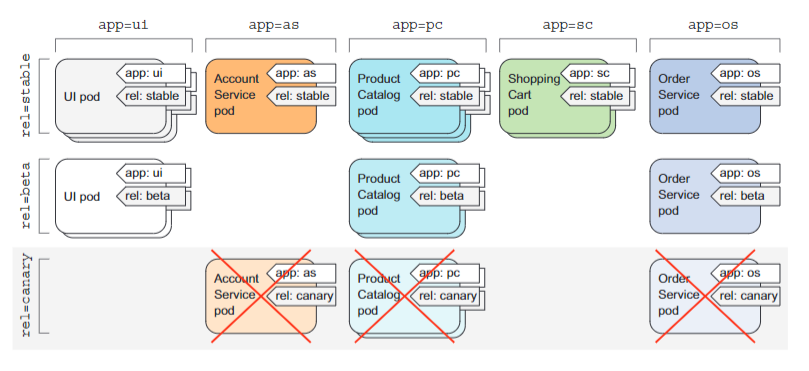
\includegraphics[width=1\textwidth]{figures/3_10.png}
		\caption{Fig. by courtesy of Marko Luksa\cite{Luksa2018}}
		\label{fig:}
	\end{figure}
}

\section[Services]{Services}
\frame{
	\frametitle{Services in Kubernetes}
	\framesubtitle{}
	Motivation
	\begin{itemize}
		\item We need a way to connect to pods from the outside.
		\item Pods are short-lived, they come and go.
		\item Clients should not know the IP's of pods.
		\item Scaling means multiple pods can provide the same service.
	\end{itemize}
	How do they work?
	\begin{itemize}
		\item A Service is a resource you create to make a single, constant point of entry to pods.
		\item Clients can now find frontend service, and frontend can find backend service.
	\end{itemize}
}

\frame{
	\frametitle{Services in Kubernetes cont.}
	\framesubtitle{}
	\begin{figure}[htbp!]
		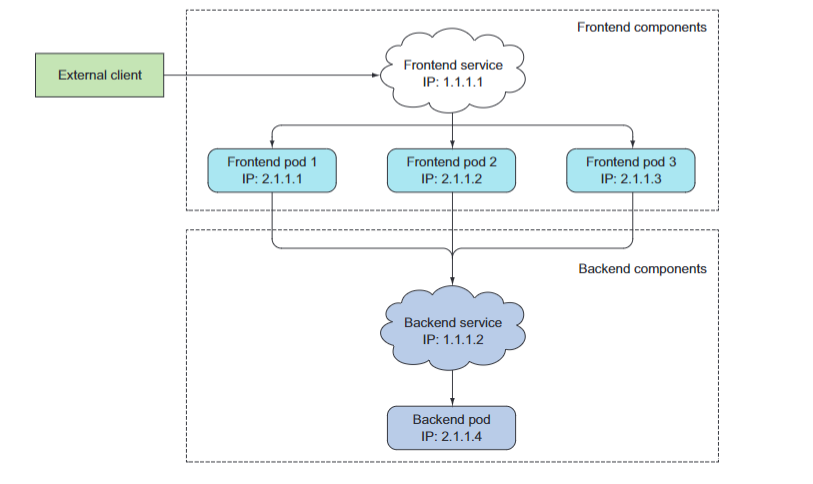
\includegraphics[width=1\textwidth]{figures/5_1.png}
		\caption{Fig. by courtesy of Marko Luksa\cite{Luksa2018}}
		\label{fig:}
	\end{figure}
}

\frame{
	\frametitle{Services in Kubernetes cont.}
	\framesubtitle{}
	\begin{figure}[htbp!]
		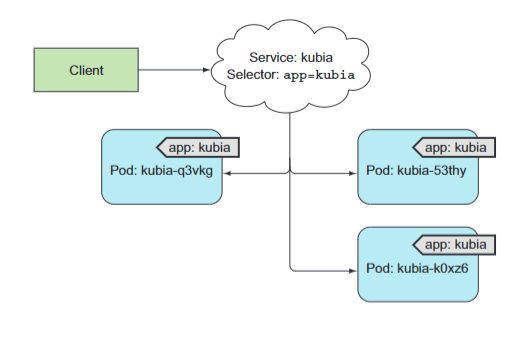
\includegraphics[width=0.9\textwidth]{figures/5_2.png}
		\caption{Fig. by courtesy of Marko Luksa\cite{Luksa2018}}
		\label{fig:}
	\end{figure}
}

\frame{
	\frametitle{Services in Kubernetes cont.}
	\framesubtitle{}
	An example of a YAML file for a service. Our service accepts connections port 80
	and route each connection to port 8080 to a pod matching \textit{app=kubia}.
	\begin{figure}[htbp!]
		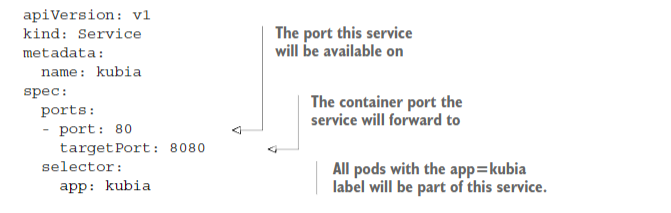
\includegraphics[width=1\textwidth]{listings/5_1.png}
		\caption{Listing by courtesy of Marko Luksa\cite{Luksa2018}}
		\label{fig:}
	\end{figure}
}

\begin{frame}[fragile]
	\frametitle{Services in Kubernetes cont.}
	\framesubtitle{}
	When created, we check to see if the service is running
	\begin{lstlisting}[numbers=none, basicstyle=\ttfamily]
$ kubectl get svc
NAME: kubia
CLUSTER-IP: 10.111.249.153
EXTERNAL-IP: <none>
PORT(S): 80/TCP
AGE: 6m
\end{lstlisting}
\end{frame}

\begin{frame}[fragile]
	\frametitle{Testing the service from the inside}
	\framesubtitle{}
	With \textit{kubectl exec} command we can access the service from inside
	Replace with your target pod and cluster IP
	\begin{lstlisting}[numbers=none, basicstyle=\ttfamily]
$ kubectl exec kubia-7nog1 -- curl -s \\
http://10.111.249.153
You've hit kubia-gzwli
	\end{lstlisting}
	The \textit{kubectl exec} behaves similarly to \textit{ssh}.
\end{frame}

\frame{
	\frametitle{Testing the service from the inside cont.}
	\framesubtitle{}
	\begin{figure}[htbp!]
		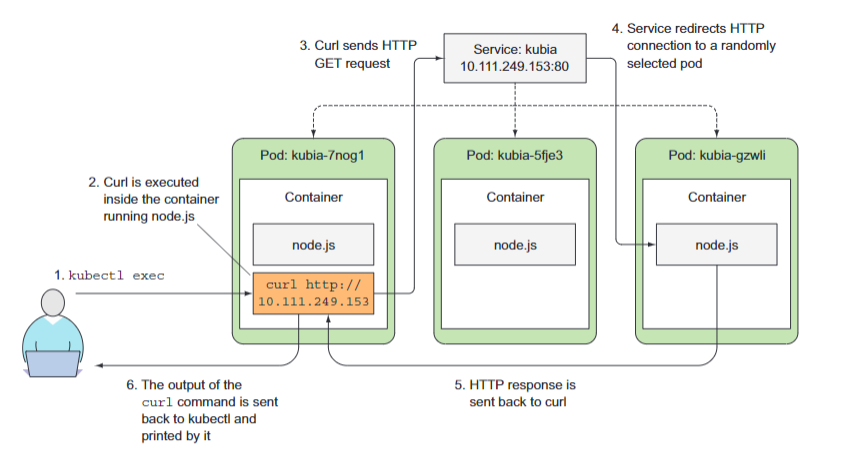
\includegraphics[width=1\textwidth]{listings/5_3.png}
		\caption{Listing by courtesy of Marko Luksa\cite{Luksa2018}}
		\label{fig:}
	\end{figure}
}

\begin{frame}[fragile]
	\frametitle{Discovering our service via DNS}
	\framesubtitle{}
	\begin{itemize}
		\item Kubernetes comes with a \textit{kube-dns} for free
		\item Each service gets a DNS entry in the internal DNS server
		\item Client pods can access the service by its FQDN.
	\end{itemize}
	\begin{lstlisting}[numbers=none, basicstyle=\ttfamily]
$ kubectl exec -it kubia-3inly
root@kubia-3inly:/#
$ curl http://kubia.default.svc.cluster.local
Youve hit kubia-5asi2
$ curl http://kubia.default
You've hit kubia-3inly
$ curl http://kubia
You've hit kubia-8awf3
	\end{lstlisting}
\end{frame}

\frame{
	\frametitle{Exposing services to external clients}
	\framesubtitle{}
	\begin{itemize}
		\item By setting the service type to NodePort (open up a port on the node itself)
		\item By setting the service type to LoadBalancer (deciated loud-balancer, AWS)
		\item By creating an Ingress resource (OSI level 7 resource)
	\end{itemize}
		\begin{figure}[htbp!]
		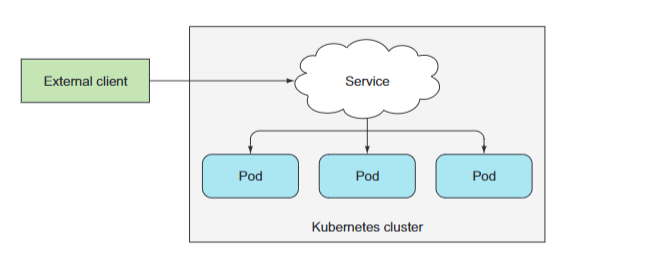
\includegraphics[width=1\textwidth]{figures/5_5.png}
		\caption{Fig. by courtesy of Marko Luksa\cite{Luksa2018}}
		\label{fig:}
	\end{figure}
}

\frame{
	\frametitle{Using a NodePort service}
	\framesubtitle{}
	\begin{itemize}
		\item For a NodePort service, each cluster node opens a port on the node itself and redirects traffic received on that port to the underlying service.
		\item This allows external traffic to our service.
		\item Can be configured with a YAML file.
	\end{itemize}
		\begin{figure}[htbp!]
		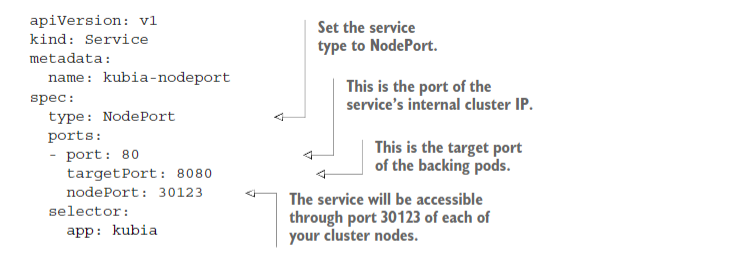
\includegraphics[width=1\textwidth]{listings/5_11.png}
		\caption{Listing by courtesy of Marko Luksa\cite{Luksa2018}}
		\label{fig:}
	\end{figure}
}

\begin{frame}[fragile]
	\frametitle{Using a NodePort service cont.}
	\framesubtitle{}
	We can check our service with \textit{kubectl get svc} command
	\begin{lstlisting}[numbers=none, basicstyle=\ttfamily]
$ kubectl get svc kubia-nodeport
NAME: kubia-nodeport
CLUSTER-IP: 10.111.254.223
EXTERNAL-IP: <nodes>
PORT(S): 80:30123/TCP
AGE: 2m
	\end{lstlisting}
The service is now accessible at the following addresses:
\begin{itemize}
	\item 10.11.254.223:80
	\item $<$1st node's IP$>$:30123
	\item $<$2nd node's IP$>$:30123, and so on.
\end{itemize}
\end{frame}

\frame{
	\frametitle{Using a NodePort service cont.}
	\framesubtitle{}
	\begin{figure}[htbp!]
		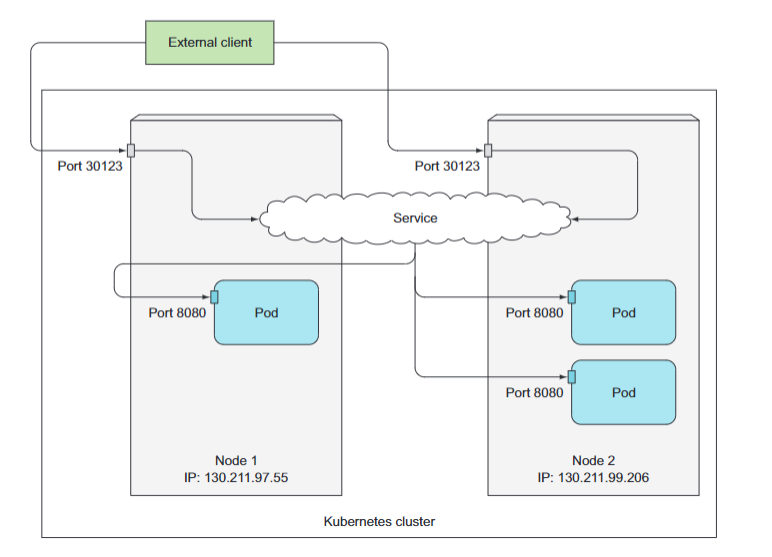
\includegraphics[width=1\textwidth]{figures/5_6.png}
		\caption{Fig. by courtesy of Marko Luksa\cite{Luksa2018}}
		\label{fig:}
	\end{figure}
}

\frame{
	\frametitle{Using a LoadBalancer service}
	\framesubtitle{}
	\begin{itemize}
		\item A LoadBalancer service is the default way to expose a service to the Internet
		\item Each service gets its own IP
		\item Was not supported by minikube until recently
		\item Available by its EXTERNAL-IP
	\end{itemize}
	\begin{figure}[htbp!]
		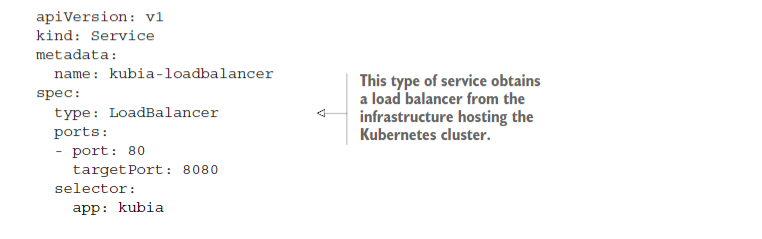
\includegraphics[width=1\textwidth]{listings/5_12.png}
		\caption{Listing by courtesy of Marko Luksa\cite{Luksa2018}}
		\label{fig:}
	\end{figure}
}

\begin{frame}[fragile]
	\frametitle{Using a LoadBalancer service cont.}
	\framesubtitle{}
	We can check our service with \textit{kubectl get svc} command
	\begin{lstlisting}[numbers=none, basicstyle=\ttfamily]
$ kubectl get svc kubia-loadbalancer
NAME: kubia-loadbalancer
CLUSTER-IP: 10.111.241.153
EXTERNAL-IP: 130.211.53.173
PORT(S): 80:32143/TCP
AGE: 1m
	\end{lstlisting}
	The service is now accessible by its external IP:\\
	curl http://130.211.53.173
\end{frame}

\frame{
	\frametitle{Using a LoadBalancer service cont.}
	\framesubtitle{}
	\begin{figure}[htbp!]
		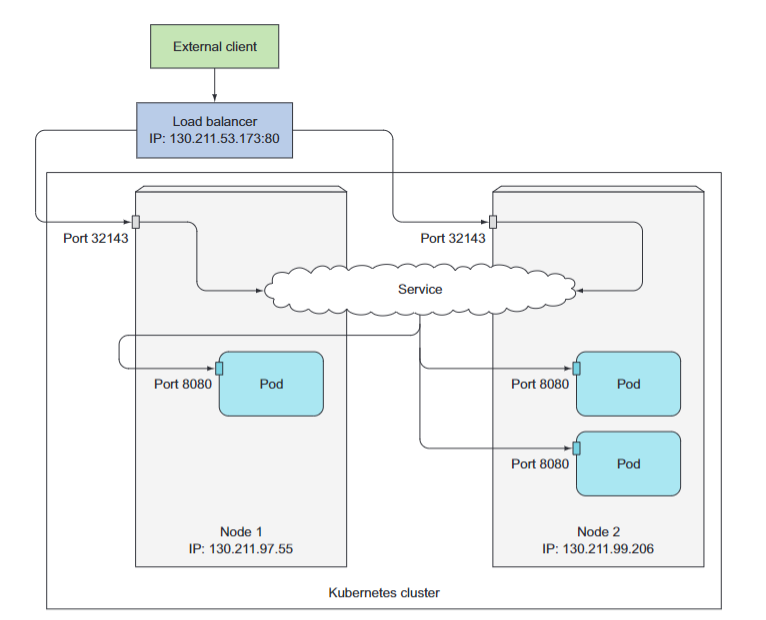
\includegraphics[width=0.7\textwidth]{figures/5_7.png}
		\caption{Fig. by courtesy of Marko Luksa\cite{Luksa2018}}
		\label{fig:}
	\end{figure}
}

\frame{
	\frametitle{Using a headless service}
	\framesubtitle{}
	Needed when client needs to connect to all pods
	\begin{itemize}
		\item A normal service just connects you to one pod
		\item A headless service will return the IP's of all annotated pods
		\item Can be accessed via DNS lookup
		\item Client libraries exist to ease communication with API
	\end{itemize}
	\begin{figure}[htbp!]
		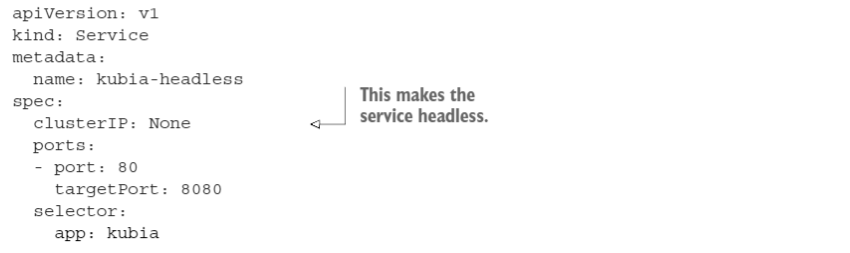
\includegraphics[width=1\textwidth]{listings/5_18.png}
		\caption{Listing by courtesy of Marko Luksa\cite{Luksa2018}}
		\label{fig:}
	\end{figure}
}

\begin{frame}[fragile]
	\frametitle{Using a headless service cont.}
	\framesubtitle{}
	We can use the dnsutils image to verify a headless service
	\begin{lstlisting}[numbers=none, basicstyle=\ttfamily]
$ kubectl run dnsutils --image=tutum/dnsutils \\
--generator=run-pod/v1 --command -- \\
sleep infinity
pod "dnsutils" created
$ kubectl exec dnsutils nslookup kubia-headless
...
Name:    kubia-headless.default ...
Address: 10.108.1.4
Name:    kubia-headless.default ...
Address: 10.108.2.5
	\end{lstlisting}
\end{frame}

\section[Deployments]{Deployments}
\frame{
	\frametitle{Deployments in Kubernetes}
	\framesubtitle{}
	What are deployments?
	\begin{itemize}
		\item A Deployment is a high-level resource
		\item It can deploy applications and update them declaratively
		\item Makes it easy to manage and make rolling-updates
		\item A Deployment is composed of a label selector,\\a replica count, and a pod template.
	\end{itemize}
	\begin{figure}[htbp!]
		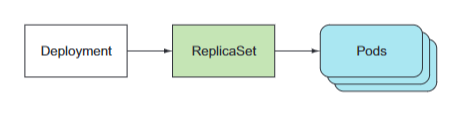
\includegraphics[width=0.8\textwidth]{figures/9_8.png}
		\caption{Fig. by courtesy of Marko Luksa\cite{Luksa2018}}
		\label{fig:}
	\end{figure}
}

\begin{frame}[fragile]
	\frametitle{Deployments in Kubernetes cont.}
	\framesubtitle{}
	\begin{figure}[htbp!]
		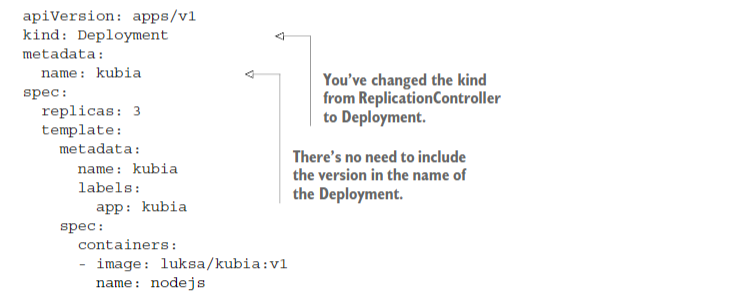
\includegraphics[width=0.9\textwidth]{listings/9_7.png}
		\caption{Listing by courtesy of Marko Luksa\cite{Luksa2018}}
		\label{fig:}
	\end{figure}
	\begin{lstlisting}[numbers=none, basicstyle=\ttfamily]
$ kubectl create -f kubia-deployment-v1.yaml
--record
$ kubectl rollout status deployment kubia
$ kubectl get po
	\end{lstlisting}
\end{frame}

\begin{frame}[fragile]
	\frametitle{Rolling out updates}
	\framesubtitle{}
	To roll-out an update, simply do
	\begin{lstlisting}[numbers=none, basicstyle=\ttfamily]
$ kubectl set image deployment kubia
nodejs=luksa/kubia:v2
	\end{lstlisting}
	\begin{figure}[htbp!]
		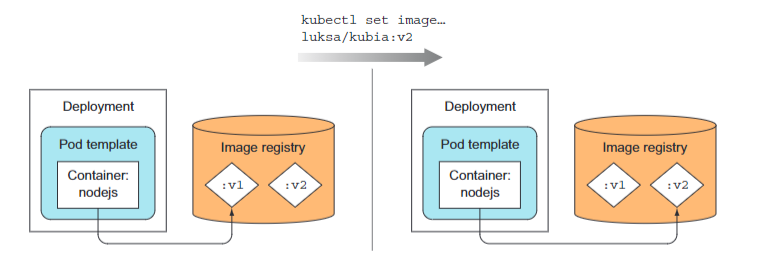
\includegraphics[width=1\textwidth]{figures/9_9.png}
		\caption{Fig. by courtesy of Marko Luksa\cite{Luksa2018}}
		\label{fig:}
	\end{figure}
\end{frame}

\frame{
	\frametitle{Rolling out updates cont.}
	\framesubtitle{}
	\begin{figure}[htbp!]
		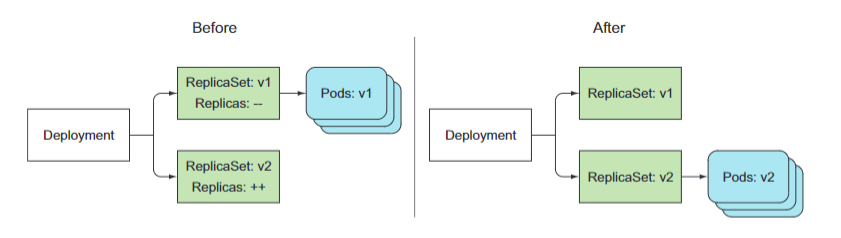
\includegraphics[width=1\textwidth]{figures/9_10.png}
		\caption{Fig. by courtesy of Marko Luksa\cite{Luksa2018}}
		\label{fig:}
	\end{figure}
}

\begin{frame}[fragile]
	\frametitle{Undoing a rollout}
	\framesubtitle{}
	Deployments make it easy to roll back an update.
	\begin{lstlisting}[numbers=none, basicstyle=\ttfamily]
$ kubectl rollout undo deployment kubia
	\end{lstlisting}
\end{frame}

\begin{frame}[fragile]
	\frametitle{View and using history}
	\framesubtitle{}
	We can check the history of our deployments
	\begin{lstlisting}[numbers=none, basicstyle=\ttfamily]
$ kubectl rollout history deployment kubia
$ kubectl rollout undo deployment kubia
--to-revision=1
	\end{lstlisting}
	\begin{figure}[htbp!]
		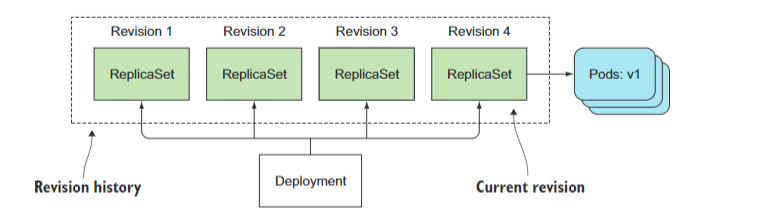
\includegraphics[width=1\textwidth]{figures/9_11.png}
		\caption{Fig. by courtesy of Marko Luksa\cite{Luksa2018}}
		\label{fig:}
	\end{figure}
\end{frame}

\frame{
	\frametitle{Control the rate of the rollout}
	\framesubtitle{}
	You can control the max surge and max unavailable pods in the Deployment manifest
	\begin{figure}[htbp!]
		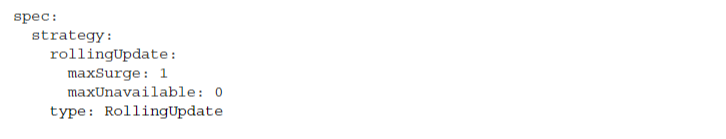
\includegraphics[width=1\textwidth]{listings/9_10.png}
		\caption{Listing by courtesy of Marko Luksa\cite{Luksa2018}}
		\label{fig:}
	\end{figure}
	\begin{itemize}
		\item maxSurge: Determines how many pods you allow to exist above
		the desired replica count. Default 25%.
		\item maxUnavailable: Determines how many pods can be unavailable relative
		to the desired replica count. Default 25%
	\end{itemize}
}

\frame{
	\frametitle{Control the rate of the rollout cont.} 
	\framesubtitle{}
	\begin{figure}[htbp!]
		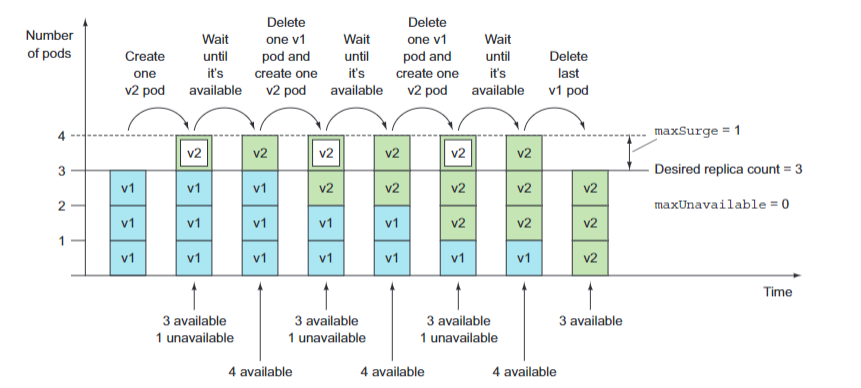
\includegraphics[width=1\textwidth]{figures/9_12.png}
		\caption{Fig. by courtesy of Marko Luksa\cite{Luksa2018}}
		\label{fig:}
	\end{figure}
}

\frame{
	\frametitle{Control the rate of the rollout cont.}
	\framesubtitle{}
	\begin{figure}[htbp!]
		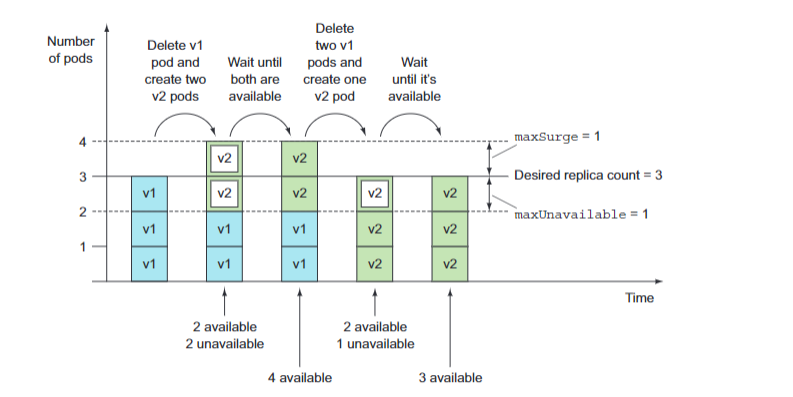
\includegraphics[width=1\textwidth]{figures/9_13.png}
		\caption{Fig. by courtesy of Marko Luksa\cite{Luksa2018}}
		\label{fig:}
	\end{figure}
}

\begin{frame}[fragile]
	\frametitle{Different ways to modify resources}
	\framesubtitle{}
	There are several ways to modify a resource in Kubernetes
	\begin{itemize}
		\item kubectl edit - Opens a object's manifest in default editor
		\item kubectl patch - Changes individual properties of an object
		\item kubectl apply - Changes or creates an object from a YAML/JSON file
		\item kubectl replace - Replaces existing object from a YAML/JSON file
		\item kubectl set image - Changes a deployment's container image
	\end{itemize}
\end{frame}


%===============References
\begin{frame}[allowframebreaks]
\frametitle{References}
%\def\section*#1{}%remove auto heading for references
\fontsize{5pt}{5pt}\selectfont
\def\newblock{\hskip .11em plus .33em minus .07em}
\bibliographystyle{chicago}
\bibliography{cl_bibliography}
\normalsize
\end{frame}

\end{document}